\documentclass[twoside]{../zirkelblatt1415}
\usepackage{mathtools}
\usepackage{wrapfig}
\usepackage{tabto}
\usepackage{booktabs}
\usepackage{relsize}
\let\raggedsection\centering

\theoremstyle{definition}
\newtheorem{defn}{Definition}[section]
\newtheorem{defn'}{Vorläufge Definition}[section]
\newtheorem{axiom}[defn]{Axiom}
\newtheorem{bsp}[defn]{Beispiel}

\theoremstyle{plain}

\newtheorem{prop}[defn]{Proposition}
\newtheorem{motto}[defn]{Motto}
\newtheorem{wunder}[defn]{Wunder}
\newtheorem{ueberlegung}[defn]{Überlegung}
\newtheorem{lemma}[defn]{Lemma}
\newtheorem{kor}[defn]{Korollar}
\newtheorem{hilfsaussage}[defn]{Hilfsaussage}
\newtheorem{satz}[defn]{Satz}
\newtheorem{thm}[defn]{Theorem}

\theoremstyle{remark}
\newtheorem{bem}[defn]{Bemerkung}
\newtheorem{warnung}[defn]{Warnung}
\newtheorem{aufg}[defn]{Aufgabe}

\definecolor{darkred}{rgb}{0.7,0,0}
\definecolor{shadecolor}{rgb}{.95,.95,.95}

\newenvironment{listing}{
  \renewcommand*\theenumi{\arabic{enumi}}
  \renewcommand{\labelenumi}{\theenumi.}
  \begin{enumerate}\itemsep0em}{\end{enumerate}}

\newcommand{\defeq}{\vcentcolon=}
\newcommand{\prim}[1]{\text{\textnormal{$#1$ prim}}}
\newcommand{\bigsum}{\mathop{\mathlarger{\mathlarger{\sum}}}}
\newcommand{\bigprod}{\mathop{\mathlarger{\mathlarger{\prod}}}}

\DeclareMathOperator{\ld}{ld}

\usepackage{mathpazo}

\begin{document}

\maketitleCustom{Klassen 10/11/12}{\textbf{\textsf{%
  Analytische Zahlentheorie \\
  \normalsize Zirkelzettel vom 5. Dezember 2014}}}

\begin{center}
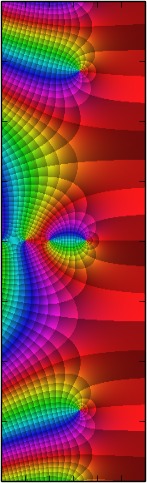
\includegraphics[angle=90]{zeta-function-complex}
\end{center}

{\renewcommand{\addvspace}[1]{\vskip0.6em}
\tableofcontents%
}

\section{Der Fundamentalsatz der Arithmetik}

\begin{defn}Eine \emph{Primzahl} ist eine positive natürliche Zahl, die
\emph{genau zwei} verschiedene positive Teiler besitzt.\end{defn}

Gemäß dieser Definition beginnt die Folge der Primzahlen also mit
\[ 2, \quad 3, \quad 5, \quad 7, \quad 11, \quad 13, \quad 17, \quad \ldots \]
Die Zahl~$1$ zählt nicht als Primzahl -- sie besitzt als einzigen Teiler sich
selbst und hat daher nicht zwei verschiedene Teiler.

\begin{thm}[Fundamentalsatz der Arithmetik]Jede positive natürliche Zahl lässt
sich auf eindeutige Art und Weise als Produkt von Primzahlen
schreiben.\end{thm}

\begin{proof}Sei eine beliebige natürliche Zahl~$n$ gegeben. Falls~$n$ eine
Primzahl ist, haben wir damit die gesuchte Zerlegung in Primfaktoren schon
gefunden. Falls~$n$ keine Primzahl ist, spaltet sich~$n$ in ein Produkt auf: $n
= a \cdot b$, und wir können mit der Suche nach einer Zerlegung bei~$a$ und~$b$
fortfahren.

Die Eindeutigkeitsaussage ist interessanter (Aufgabe~\ref{aufg:eindt}).\end{proof}

\begin{aufgabe}{Primfaktorzerlegung der Eins}
Der Fundamentalsatz der Arithmetik behauptet, dass sich \emph{jede} positive
natürliche Zahl in Primfaktoren zerlegen lässt. Die Zahl~$1$ ist auch eine
solche positive natürliche Zahl. Siehst du, wie sich diese zerlegen lässt?

\emph{Hinweis.} Das ist etwas versteckt. Beachte, dass~$1$ keine Primzahl ist.
\end{aufgabe}

\begin{aufgabe}{Soll Eins eine Primzahl sein?}
Es gibt ein gutes mathematisches Argument, wieso es sinnvoll ist, die Eins
nicht als Primzahl zu definieren. Finde es!

\emph{Tipp.} Denke an die Eindeutigkeit der Primfaktorzerlegung. Was wäre, wenn
man die Zahl Eins als Primzahl zulassen würde?
\end{aufgabe}

\begin{aufgabe}{Eindeutigkeit der Primfaktorzerlegung}\label{aufg:eindt}
Mit dieser Aufgabe beweisen wir, dass die Zerlegung einer Zahl in Primfaktoren
bis auf Umordnung der Faktoren eindeutig ist. In Formeln ausgedrückt: Gilt
\[ p_1 \cdots p_n = q_1 \cdots q_m, \]
wobei~$p_1,\ldots,p_n$ und~$q_1,\ldots,q_m$ Primzahlen sind, so folgt schon~$n
= m$ (links und rechts stehen also gleich viele Faktoren) und jeder Faktor der
linken Seite tritt auch genau einmal auf der rechten Seite auf und umgekehrt.

\begin{enumerate}
\item Zeige zuerst: Teilt eine Primzahl~$p$ ein Produkt~$a \cdot b$, so
teilt~$p$ schon~$a$ oder~$p$ teilt~$b$. In Formeln:
\[ \text{Wenn $p \mid ab$, dann $p \mid a$ oder $p \mid b$.} \]

\emph{Tipp.} Das ist gar nicht so leicht. Verwende, dass die Zahlen~$a$ und~$p$
irgendeinen größten gemeinsamen Teiler~$d$ haben, und dass sich dieser in der
Form~$d = fa + gp$ für gewisse Zahlen~$f$ und~$g$ schreiben lässt. (Eine solche
Darstellung des größten gemeinsamen Teilers heißt \emph{Bézoutdarstellung}.
Dass es eine solche immer gibt, folgt aus dem \emph{euklidischen Algorithmus}.)

\item Beweise mit dem Resultat aus Teilaufgabe~a) die Eindeutigkeitsbehauptung.
\end{enumerate}\fixlistspacing
\end{aufgabe}

\begin{aufgabe}{Primzahlen mögen Vielfache der Sechs}
Beweise: Jede Primzahl größer als~$3$ liegt benachbart zu einem Vielfachen
von~$6$. In Formeln: Ist~$p > 3$ eine Primzahl, so teilt~$6$ entweder~$p-1$
oder~$p+1$.

\emph{Tipp.} Eine Zahl ist genau dann ein Vielfaches von~$6$, wenn sie ein
Vielfaches von~$2$ und von~$3$ ist. Weißt du von den drei Zahlen~$p-1$,~$p$
und~$p+1$, ob sie ein Vielfaches von~$3$ sind?
\end{aufgabe}


\section{Die Entdeckung der Irrationalität}

\begin{defn}Eine reelle Zahl~$x$ heißt genau dann \emph{rational}, wenn sie
sich als Quotient zweier ganzer Zahlen schreiben lässt: $x = a/b$ für gewisse
ganze Zahlen~$a$ und~$b$.\end{defn}

Dass nicht alle Zahlen rational sind, war eine erstaunliche Entdeckung im
fünften Jahrhundert~v.~Chr. Manche sehen diese Erkenntnis sogar als
Geburtsstunde der modernen Mathematik an. Als Entdecker der
Irrationalität gilt der griechische Mathematiker Hippasos von Metapont. Er
erkannte, dass der \emph{goldene Schnitt} irrational ist. Damit erschütterte er
die Schule der Pythagoreer, denn diese waren von dem Kredo \emph{Alles ist
Zahl} überzeugt, wobei sie mit "`Zahl"' \emph{rationale Zahl} meinten.
Ironischerweise kam der goldene Schnitt auch noch im Erkennungszeichen der
Pythagoreer vor, dem Pentagramm.

\begin{thm}Die Zahl~$\sqrt{2}$ ist nicht rational.\end{thm}

\begin{aufgabe}{Irrationalität von Quadratwurzeln}
\begin{enumerate}
\item Beweise, dass~$\sqrt{2}$ nicht rational ist.

\emph{Tipp.} Gehe nach folgendem Muster vor. Angenommen,~$\sqrt{2}$ ist doch
rational. Nach Definition gibt es dann ganze Zahlen~$a$ und~$b$ mit~$\sqrt{2} =
a/b$. Quadrieren und Umstellen zeigt~$2 b^2 = a^2$. Überlege nun, wie oft der
Primfaktor~$2$ auf den beiden Seiten dieser Gleichung vorkommt.

\item Beweise, dass für jede Primzahl~$p$ die Zahl~$\sqrt{p}$ nicht rational
ist.

\item Beweise, dass für jede Zahl~$n$, in deren Primfaktorzerlegung mindestens
eine Primzahl ungerade oft vorkommt, die Zahl~$\sqrt{n}$ nicht rational ist.
\end{enumerate}\fixlistspacing
\end{aufgabe}

\begin{aufgabe}{Anschauliche Bedeutung von Quadratwurzeln}
Wenn Quadratwurzeln sehr seltsame Zahlen ohne praktische Bedeutung wären,
hätte die Entdeckung der Irrationalität vielleicht einen geringeren
Stellenwert. Tatsächlich aber kommen Quadratwurzeln in der
Geometrie überall vor: Finde eine geometrische Figur, deren Kantenlängen alle
ganze Zahlen sind, sodass eine weitere eingezeichnete Hilfslinie aber
irrationale Länge hat.
\end{aufgabe}

\begin{aufgabe}{Irrationalität des goldenen Schnitts}
Der \emph{goldene Schnitt} ist diejenige positive Zahl~$\phi$, die die
Gleichung~$\phi = 1 + \frac{1}{\phi}$ löst. Als Schnittverhältnis kommt der goldene
Schnitt überall in der Natur vor.

\begin{enumerate}
\item Beweise rechnerisch, dass der goldene Schnitt irrational ist.

\emph{Tipp.} Gehe nach folgendem Muster vor. Angenommen,~$\phi$ ist rational.
Dann lässt sich~$\phi$ als ein vollständig gekürzter Bruch~$\phi = a/b$
schreiben. Zähler und Nenner sind dabei zueinander teilerfremde Zahlen. Welche
Beziehung erhält man zwischen~$a$ und~$b$, wenn man~$\phi = a/b$ in die
Gleichung~$\phi = 1 + 1/\phi$ einsetzt?

\item In dem Skript von Jost-Hinrich Eschenburg zu seiner letzten
Vorlesungsreihe, den \emph{Sternstunden} (die du auch besuchen kannst, wenn du
möchtest: jeden Freitag um 12:15~Uhr), findest du auch einen geometrischen
Beweis der Irrationalität des goldenen Schnitts sowie eine Erklärung, wieso der
goldene Schnitt die \emph{irrationalste} Zahl ist.
\url{http://www.math.uni-augsburg.de/~eschenbu/sternstunden.pdf}
\end{enumerate}\fixlistspacing
\end{aufgabe}


\section{Die Unendlichkeit der Primzahlen}

Es gibt unendlich viele Primzahlen. Es ist bemerkenswert, dass wir das rigoros
beweisen können -- obwohl wir natürlich niemals alle Primzahlen aufschreiben
können.

\begin{thm}Zu jeder endlichen Liste von Primzahlen gibt es eine weitere
Primzahl, die nicht in der Liste enthalten ist.\end{thm}

\begin{aufgabe}{Euklids Beweis der Unendlichkeit der Primzahlen}
\label{aufg:unendlich-euklid}
Seien~$p_1,\ldots,p_n$ irgendwelche Primzahlen. Wir suchen eine weitere
Primzahl, die ungleich den gegebenen Primzahlen ist. Dazu betrachten wir die
Hilfszahl
\[ N \defeq \prod_{i=1}^n p_i + 1 = p_1 p_2 \cdots p_{n-1} p_n + 1. \]
\begin{enumerate}
\item Wieso teilt keine der gegebenen Primzahlen~$p_1,\ldots,p_n$ die Zahl~$N$?
\item Wie erhält man aus~$N$ also eine neue Primzahl, die ungleich den
gegebenen ist?
\end{enumerate}

\emph{Bemerkung.} Euklids Argumentation wird gelegentlich auch in
Widerspruchsbeweisen verwendet, in deren Kontext die hier definierte Zahl~$N$
dann stets eine Primzahl ist. Im Allgemeinen ist~$N$ aber keine Primzahl. Etwa
sind~$3 \cdot 5 + 1 = 16$ und~$2 \cdot 3 \cdot 5 \cdot 7 \cdot 11 \cdot 13 + 1
= 30031 = 59 \cdot 509$ keine Primzahlen.
\end{aufgabe}


\section{\texorpdfstring{Die Riemannsche~$\boldsymbol{\zeta}$-Funktion}{Die
Riemannsche~ζ-Funktion}}

\begin{defn}Für reelle Zahlen~$s > 1$ ist die \emph{Riemannsche
$\zeta$-Funktion} durch folgende Formel definiert.
\[ \zeta(s) \defeq \sum_{n=1}^\infty \frac{1}{n^s} =
  \frac{1}{1^s} + \frac{1}{2^s} + \frac{1}{3^s} + \frac{1}{4^s} + \cdots \]
\end{defn}

\setlength{\wrapoverhang}{1cm}
\setlength{\columnsep}{0.5cm}
\begin{wrapfigure}{r}{0.25\textwidth}
\vspace{-4em}
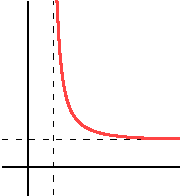
\includegraphics[scale=1]{zeta-function-real}
\end{wrapfigure}
Die Riemannsche~$\zeta$-Funktion ist also durch eine \emph{unendliche Reihe}
festgelegt. Je nachdem, wie schnell die Summanden einer unendlichen Reihe gegen
Null streben, hat sie entweder einen richtigen Zahlenwert (sie
\emph{konvergiert}), den Wert~$+\infty$ oder den Wert~$-\infty$ (sie
\emph{divergiert bestimmt}) oder gar keinen Wert (sie \emph{divergiert
unbestimmt}). Mit Reihen, die nicht konvergieren, kann man nicht wie gewöhnlich
rechnen -- das soll Aufgabe~\ref{aufg:grandi} demonstrieren. Mit dem
\emph{Integralvergleichskriterium}, das man im ersten Semester eines
Mathe-Studiums lernt, kann man aber leicht nachweisen, dass für~$s > 1$ die
gegebene Reihe konvergiert.

Der reelle Graph der~$\zeta$-Funktion ist sehr unspektakulär. Er hat
die Geraden~$x = 1$ und~$y = 1$ als Asymptoten.
So unscheinbar dieser Graph und die Definition auch sein mögen, die Riemannsche~$\zeta$-Funktion
hat eine Vielzahl kurioser Eigenschaften und ist Gegenstand vieler
mathematischer Vermutungen. In der analytischen Zahlentheorie ist sie von
fundamentaler Bedeutung, angewendet wird sie aber auch in Physik,
Wahrscheinlichkeitstheorie und Statistik.

\begin{itemize}
\item Die~$\zeta$-Funktion lässt sich auch als ein zahlentheoretisches
interessantes Produkt schreiben (Abschnitt~\ref{sect:euler-produkt}).
\item Für~$s \to 1$ divergiert~$\zeta(s)$. Das ist eng mit der Unendlichkeit
der Primzahlen verbunden.
\item Es ist schwierig, geschlossene Ausdrücke für Funktionswerte
der~$\zeta$-Funktion anzugeben. Aber beispielsweise gilt~$\zeta(2) = \pi^2/6$.
Die Funktionswerte an allen anderen positiven geraden Zahlen~$n$ sind ebenfalls
bekannt, sie sind wie~$\zeta(2)$ bestimmte rationale Vielfache von~$\pi^n$.
\item Man vermutet, dass die Werte der~$\zeta$-Funktion an allen positiven
ungeraden Zahlen (außer der Eins) irrational sind. Man weiß schon, dass zumindest unendlich
viele dieser Werte irrational sind, und man weiß auch, dass~$\zeta(3)$
irrational ist. Es ist aber noch nicht einmal bekannt, ob auch~$\zeta(5)$ irrational
ist. (Kurioserweise weiß man aber, dass unter den Zahlen~$\zeta(5)$,
$\zeta(7)$, $\zeta(9)$ und~$\zeta(11)$ mindestens eine irrational sein muss.)
\item Obwohl die definierende Formel nur für~$s > 1$ konvergiert, lässt sich
die~$\zeta$-Funktion auf den Bereich~$s < 1$ und sogar auf \emph{alle komplexen
Zahlen} ungleich~$1$ fortsetzen.
\item Die Werte der~$\zeta$-Funktion an allen negativen ganzen Zahlen sind
bekannt. Bei allen negativen geraden Zahlen hat sie Nullstellen, die so
genannten \emph{trivialen Nullstellen der~$\zeta$-Funktion}.
\item Es ist bekannt, dass alle weiteren Nullstellen in den komplexen Zahlen
Realteil zwischen~$0$ und~$1$ (jeweils ausgeschlossen) haben.
\item Man vermutet, dass diese so genannten \emph{nichttrivialen Nullstellen}
sogar alle Realteil genau~$1/2$ haben. Das besagt die berühmte \emph{Riemannsche
Vermutung}.
\item Die Riemannsche Vermutung ist eng verwandt mit der Verteilung der
Primzahlen und der Goldbachschen Vermutung. Eine lange Liste von Konsequenzen
der Riemannschen Vermutung gibt es auf
\url{http://mathoverflow.net/questions/17209/consequences-of-the-riemann-hypothesis}.
\end{itemize}

\begin{aufgabe}{Eine einfache konvergente Reihe}\label{aufg:konvergente-reihen}
\begin{enumerate}
\item Was ergibt~$1 + 0{,}1 + 0{,}01 + 0{,}001 + \cdots$?
\item Was ergibt~$1 + 0{,}1_2 + 0{,}01_2 + 0{,}001_2 + \cdots$, wenn man die
Summanden im Binärsystem liest?
\end{enumerate}\fixlistspacing
\end{aufgabe}

\begin{aufgabe}{Grandis Reihe}\label{aufg:grandi}
Sei~$s \defeq 1 - 1 + 1 - 1 + \cdots$. Diese Reihe divergiert, man kann mit ihr
nicht wie gewöhnlich rechnen. Das sollen die folgenden Teilaufgaben
illustrieren. Die Reihe ist nach dem italienischen Mathematiker und
Geistlichen Guido Grandi (*~1671, †~1742) benannt.
\begin{enumerate}
\item Fasse die ersten beiden Summanden zusammen, dann die zweiten beiden, die
dritten beiden, und so weiter. Welches Ergebnis erhält man auf diese Art und
Weise für~$s$?
\item Lass den ersten Summanden vorne stehen, fasse dann aber den zweiten und
dritten Summanden zusammen, den vierten und fünften, und so weiter. Was
ist nun das Ergebnis?
\item Wie muss man die Summanden zusammenfassen, um deine Lieblingszahl als
Ergebnis zu erhalten?
\item Finde einen Weg, um die Gleichung~$1 - s = s$ nicht unplausibel zu
finden. Welchen Wert hat~$s$ dieser Gleichung zufolge?
\end{enumerate}\fixlistspacing
\end{aufgabe}

\begin{aufgabe}{Was ist~$\zeta(2)$?}\label{aufg:zeta2}
Die Zahl~$\zeta(2)$ ist gleich~$\pi^2/6$. Der übliche Beweis dieser Tatsache
verwendet mehrdimensionale Integrationstheorie und erfordert daher mehr
Vorkenntnisse, als wir hier voraussetzen möchten. Es ist aber auch schon spannend
zu verstehen, wieso~$\zeta(2)$ überhaupt \emph{endlich} ist. Das ist ja,
angesichts der Definition von~$\zeta(2)$ als die unendliche Reihe
\[ \zeta(2) = \frac{1}{1} + \frac{1}{4} + \frac{1}{9} + \frac{1}{16} + \cdots,
\]
gar nicht klar.
\begin{enumerate}
\item Finde zunächst den Wert von
\[ \sum_{n=2}^\infty \frac{1}{(n-1) \cdot n} =
  \frac{1}{1 \cdot 2} + \frac{1}{2 \cdot 3} + \frac{1}{3 \cdot 4} + \cdots. \]

\emph{Tipp.} Rechne nach, dass gilt: $\frac{1}{(n-1) \cdot n} = \frac{1}{n-1} -
\frac{1}{n}$. Mit dieser Erkenntnis kannst du die Summe umschreiben und
ausrechnen. Dabei wirst du feststellen, dass sich die meisten Summanden
gegenseitig wegheben; Summen, bei denen das passiert, heißen auch
\emph{Teleskopsummen}.

\item Zeige: $\zeta(2) < \infty$.

\emph{Tipp.} In welchem Größenverhältnis stehen~$\frac{1}{n^2}$
und~$\frac{1}{(n-1) \cdot n}$ zueinander?
\end{enumerate}\fixlistspacing
\end{aufgabe}


\section{Die Eulersche Produktformel}\label{sect:euler-produkt}

\begin{thm}Für alle~$s > 1$ gilt die Identität
\[ \zeta(s) = \bigprod_{\substack{p\\\prim{p}}} \frac{1}{1 - p^{-s}} =
  \frac{1}{1 - 2^{-s}} \cdot \frac{1}{1 - 3^{-s}} \cdot \frac{1}{1 - 5^{-s}} \cdots. \]
\end{thm}
Diese Beziehung ist aus mehreren Gründen bemerkenswert. Zunächst einmal ist es
eine Seltenheit, dass sich eine \emph{Summe} (die linke Seite der Gleichung)
auch als ein (nichttriviales) \emph{Produkt} schreiben lässt. Zudem noch gehen
in die rechte Seite die Primzahlen ein, beim bloßen Anblick der Formel für
die~$\zeta$-Funktion würde man das nicht vermuten.

Für den Beweis benötigen wir die Formel für die \emph{geometrische Reihe}
(Aufgabe~\ref{aufg:geometrische-reihe}),
\[ \sum_{m = 0}^\infty x^m = 1 + x + x^2 + x^3 + \cdots = \frac{1}{1 - x}, \]
und die Potenzgesetze~$x^{-a} = 1/x^a$ sowie~$(x^a)^b = x^{ab}$.

\begin{proof}Wir beginnen mit der rechten Seite der Gleichung. Der Bruch passt
auf die Formel für die geometrische Reihe, deswegen gilt
\[
  \bigprod_{\substack{p\\\prim{p}}} \frac{1}{1 - p^{-s}} =
  \bigprod_{\substack{p\\\prim{p}}} \left(1 + p^{-s} + (p^2)^{-s} + \cdots\right).
\]
Wenn wir dieses unendliche Produkt ausmultiplizieren, erhalten wir
die Summe über alle Zahlen der Form~$1/t^s$, wobei~$t$ alle Möglichkeiten,
beliebig viele Primzahlen aufzumultiplizieren, durchläuft. Da sich nach dem
Fundamentalsatz der Arithmetik jede positive natürliche Zahl auf genau eine Art
und Weise als Produkt von Primzahlen schreiben lässt, erhalten wir also die
Summe über alle Zahlen der Form~$1/n^s$, wobei~$n$ alle positiven natürlichen
Zahlen durchläuft. Nach Definition ist diese Summe~$\zeta(s)$.
\end{proof}

Überblick verloren? Aufgabe~\ref{aufg:euler-produkt} wird in kleinen handlichen
Stücken den Beweis verständlich machen.

\begin{aufgabe}{Die geometrische Reihe}\label{aufg:geometrische-reihe}
In dieser Aufgabe wollen wir die so genannte \emph{geometrishe Reihe}
\[ s \defeq 1 + x + x^2 + x^3 + \cdots \]
auswerten. Der erste Schritt dazu ist mit dieser Zeile schon getan -- in der
Mathematik wird vieles einfacher, wenn man dem Unbekannten einen Namen
gibt:~$s$. Denn dann steht der Weg für algebraische Umformungen offen.
\begin{enumerate}
\item Rechne nach: $s \cdot (1 - x) = 1$.

\emph{Tipp.} Multipliziere die unendliche Summe aus.

\item Folgere: $s = 1/(1-x)$.

\item Löse Aufgabe~\ref{aufg:konvergente-reihen} erneut, und zwar unter
Verwendung der Formel aus~b).
\end{enumerate}

\emph{Bemerkung.} Die Multiplikation mit~$(1-x)$, die zur Auswertung von~$s$
also sehr hilfreich war, war ein \emph{Trick}. Der Definition von~$s$ ist
dieser nicht zu entnehmen, man benötigt Kreativität und Geduld, um auf ihn zu
kommen. Die geometrische Reihe konvergiert nur, falls der Betrag von~$s$
kleiner als~$1$ ist, und nur in diesem Fall gilt die Formel~$s = 1/(1-x)$.
Diese Subtilitäten wollen wir nicht weiter beachten, obwohl sie durchaus
wichtig sind.
\end{aufgabe}

\begin{aufgabe}{Beweise ohne Worte}
Die aus dem Internet ausgeliehenen Skizzen demonstrieren (von links
nach rechts) folgende Sachverhalte -- und zwar ganz ohne
Formeln und Rechnungen. Schaue dir die Skizzen lang genug an, um zu verstehen,
wieso sie diese Sachverhalte wirklich beweisen.
\begin{multicols}{2}
\begin{enumerate}
\item $\frac{1}{4} + \left(\frac{1}{4}\right)^2 + \left(\frac{1}{4}\right)^3 +
\cdots = \frac{1}{3}$.
\item Wie bei~a).
\item $\frac{1}{3} + \left(\frac{1}{3}\right)^2 + \left(\frac{1}{3}\right)^3 +
\cdots = \frac{1}{2}$.
\item $\frac{1}{2} + \left(\frac{1}{2}\right)^2 + \left(\frac{1}{2}\right)^3 +
\cdots = 1$.
\end{enumerate}
\end{multicols}
\begin{center}
  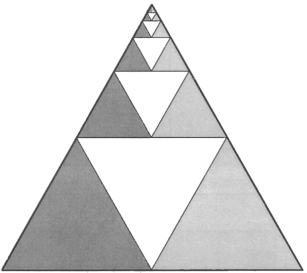
\includegraphics[height=0.2\textwidth]{geometrische-reihe-1}\quad
  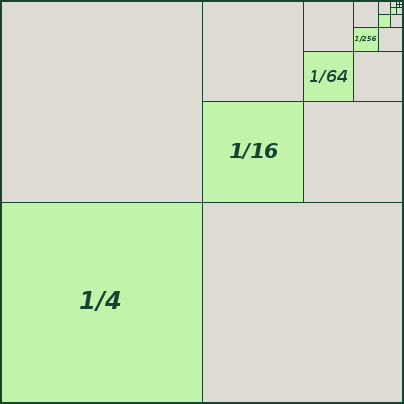
\includegraphics[height=0.2\textwidth]{geometrische-reihe-2}\quad
  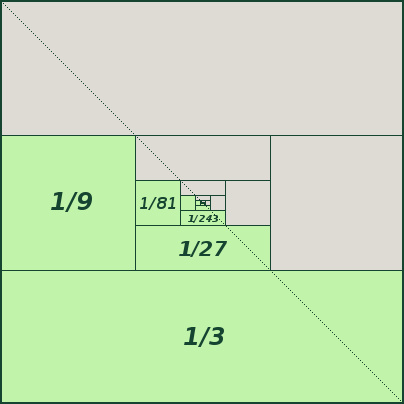
\includegraphics[height=0.2\textwidth]{geometrische-reihe-3}\quad
  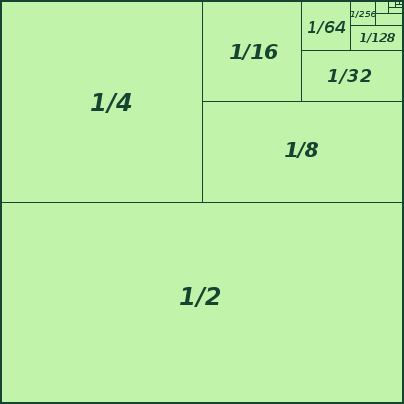
\includegraphics[height=0.2\textwidth]{geometrische-reihe-4}
\end{center}
Es ist sogar möglich, die allgemeine Formel für die geometrische Reihe aus
Aufgabe~\ref{aufg:geometrische-reihe} durch eine aussagekräftige Skizze zu
beweisen. Kannst du erklären, wie das funktioniert? (Achtung, knifflig!)
\begin{center}
  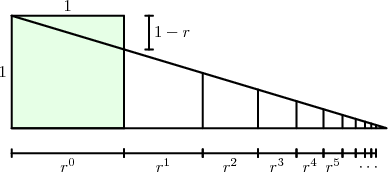
\includegraphics[scale=0.5]{geometrische-reihe-6}
\end{center}
\end{aufgabe}

\begin{aufgabe}{Die Eulersche Produktformel in fünf Schritten}
\label{aufg:euler-produkt}
\begin{enumerate}
\item Zum Aufwärmen: Multipliziere folgendes Produkt aus.
\[ \left(1 + \frac{1}{2} + \frac{1}{2^2}\right) \cdot
  \left(1 + \frac{1}{3} + \frac{1}{3^2}\right). \]
\item Multipliziere jetzt in dem Produkt
\[ \left(1 + \frac{1}{2} + \frac{1}{2^2} + \frac{1}{2^3} + \cdots\right) \cdot
  \left(1 + \frac{1}{3} + \frac{1}{3^2} + \frac{1}{3^3} + \cdots\right) \]
die Klammern so lange aus, bis du genug von dem System verstehst, um zu
erkennen: Hier kommt die Summe über die Kehrwerte von all den positiven
natürlichen Zahlen, in deren Primfaktorzerlegung nur die Faktoren~$2$ und~$3$
auftreten, heraus.
\item Multipliziere nun das dreifache Produkt
\[ \left(1 + \frac{1}{2} + \frac{1}{2^2} + \cdots\right) \cdot
  \left(1 + \frac{1}{3} + \frac{1}{3^2} + \cdots\right) \cdot
  \left(1 + \frac{1}{5} + \frac{1}{5^2} + \cdots\right) \]
soweit aus, um zu erkennen, dass das die Summe über die Kehrwerte von all den
positiven natürlichen Zahlen, in deren Primfaktorzerlegung nur die Faktoren~$2$,~$3$
und~$5$ vorkommen, ergibt.
\item Mit dieser Vorarbeit ist es nicht mehr schwer, zu glauben, dass das
unendliche Produkt
\[ \left(1 + \frac{1}{2} + \frac{1}{2^2} + \cdots\right)
  \left(1 + \frac{1}{3} + \frac{1}{3^2} + \cdots\right)
  \left(1 + \frac{1}{5} + \frac{1}{5^2} + \cdots\right) \cdots \]
gleich der Summe über die Kehrwerte von \emph{allen} positiven natürlichen Zahlen ist.
\item Schlussendlich: Ergänzen wir überall ein "`hoch~$s$"', so erhalten wir
die Summe über alle Zahlen der Form~$1/n^s$, wobei~$n$ über alle positiven
natürlichen Zahlen läuft. Das ist die Eulersche Produktformel.
\[\textstyle \left(1 + \frac{1}{2^s} + \frac{1}{(2^2)^s} + \cdots\right)
  \left(1 + \frac{1}{3^s} + \frac{1}{(3^2)^s} + \cdots\right)
  \left(1 + \frac{1}{5^s} + \frac{1}{(5^2)^s} + \cdots\right) \cdots =
  \sum_{n=1}^\infty \frac{1}{n^s}. \]
\end{enumerate}\fixlistspacing
\end{aufgabe}


\section{Die harmonische Reihe}
\label{sect:harmonische-reihe}

Die unendliche Reihe
\[ \frac{1}{1} + \frac{1}{2} + \frac{1}{3} + \frac{1}{4} + \cdots \]
wird \emph{harmonische Reihe} genannt. Sie divergiert bestimmt, ihr Wert
ist~$+\infty$.

Mit ein wenig Hintergrundwissen aus Integrationstheorie kann man sich
überlegen, dass die harmonische Reihe in etwa so schnell wächst wie der
natürliche Logarithmus:
\begin{equation}
  \label{star}
  \tag{$\star$}
  \frac{1}{1} + \frac{1}{2} + \cdots + \frac{1}{n} \approx \ln(n),
\end{equation}
und eine verfeinerte Analyse liefert folgendes Resultat.

\begin{thm}Es gibt eine Konstante~$\gamma \approx 0{,}57722$, die
\emph{Euler--Mascheroni-Konstante}, der sich die Differenzen aus linker und
rechter Seite von~\eqref{star} beliebig genau nähern. In Symbolen:
\[ \sum_{i=1}^n \frac{1}{i} - \ln(n) \xrightarrow{n \to \infty}
\gamma. \]
\end{thm}

In diesem Kontext gibt es eine Abschätzung, die für unsere Zwecke wichtig sein wird:
\[ \sum_{i=1}^{\lceil e^{A-\gamma} \rceil} \tfrac{1}{i} > A. \]
Die Klammern bezeichnen dabei die \emph{Aufrundungsoperation}.

\begin{center}\begin{tabular}{rrrr}
  \toprule
  $A$ & $e^{A-\gamma}$ & $\lceil e^{A-\gamma} \rceil$ & $\sum_{i=1}^{\lceil e^{A-\gamma} \rceil} 1/i$ \\\midrule
   1 &     1.56 &     2 &  1.50 \\
   2 &     4.23 &     5 &  2.28 \\
   3 &    11.50 &    12 &  3.10 \\
   4 &    31.26 &    32 &  4.06 \\
   5 &    84.97 &    85 &  5.03 \\
   6 &   230.97 &   231 &  6.02 \\
   7 &   627.84 &   628 &  7.02 \\
   8 &  1706.63 &  1707 &  8.02 \\
   9 &  4639.11 &  4640 &  9.02 \\
  10 & 12610.42 & 12611 & 10.02 \\
  \bottomrule
\end{tabular}\end{center}

\begin{aufgabe}{Divergenz der harmonischen Reihe}
\begin{enumerate}
\item Wieso ist~$\frac{1}{3} + \frac{1}{4} \geq \frac{1}{2}$?
\tabto{6cm}
\emph{Tipp.} $\frac{1}{3} \geq \frac{1}{4}$ und~$\frac{1}{4} + \frac{1}{4} =
\frac{1}{2}$.
\item Wieso ist~$\frac{1}{5} + \frac{1}{6} + \frac{1}{7} + \frac{1}{8} \geq \frac{1}{2}$?
\tabto{6cm}
\emph{Tipp.} $\frac{1}{5}, \frac{1}{6}, \frac{1}{7} \geq \frac{1}{8}$.

\item Wieso ist~$\frac{1}{9} + \cdots + \frac{1}{16} \geq \frac{1}{2}$?

\item Wieso ist~$\frac{1}{17} + \cdots + \frac{1}{32} \geq \frac{1}{2}$?

\item Folgere: Die harmonische Reihe ist größergleich
$\frac{1}{1} + \frac{1}{2} + \frac{1}{2} + \frac{1}{2} + \cdots$,
und das ist sicherlich~$+\infty$.
\end{enumerate}\fixlistspacing
\end{aufgabe}

\begin{aufgabe}{Slow harmonic series is slow}
Die harmonische Reihe divergiert zwar, tut das aber sehr langsam. Addiere mit
einem Taschenrechner oder einem Computerprogramm so viele Terme der Reihe, wie
du möchtest. Ich wette, du wirst nicht über~$30$ hinauskommen.
\end{aufgabe}

\begin{aufgabe}{Eulers Beweis der Unendlichkeit der Primzahlen}
\begin{enumerate}
\item Was ist~$\zeta(1)$?
\item Verwende Eulers Produktformel, um einen alternativen Beweis der
Unendlichkeit der Primzahlen zu führen: Wie sähe die Formel aus, wenn es nur
endlich viele Primzahlen gäbe?
\end{enumerate}\fixlistspacing
\end{aufgabe}


\section{Grobe Schranken für die Größen der Primzahlen}

Es gibt keine geschlossene Formel für die Primzahlen.\footnote{Das ist nur halb
wahr. Informiere dich über \emph{Mills Formel}.} Trotzdem kann man explizite
\emph{Schranken} für die Größe der~$n$-ten Primzahl angeben. Mit deren Hilfe
kann man angeben, wie viele Primzahlen es in einem vorgegebenem Bereich
mindestens geben muss oder höchstens geben kann.

Ein erstes Resultat in diese Richtung ist das folgende. Dabei
sei~$p_1,p_2,p_3,\ldots$ die unendliche Liste aller Primzahlen.

\begin{thm}\label{thm:schranke1}\ \\[-2em]
\begin{enumerate}
\item
Ist~$p$ eine Primzahl, so ist die nächste Primzahl~$\leq p! + 1$. \\[-2em]
\item
Die~$r$-te Primzahl ist höchstens~$2^{(2^r)}$: $p_r < 2^{(2^r)}$.
\end{enumerate}
\end{thm}

Das folgende Resultat ist schwieriger zu beweisen, liefert aber auch eine
bessere (kleinere) Abschätzung. Die Klammern bezeichnen wieder die
Aufrundungoperation.

\begin{thm}\label{thm:schranke2}\ \\[-2em]
\begin{enumerate}
\item
Ist~$p$ eine Primzahl, so ist die nächste Primzahl~$\leq \lceil e^{p-\gamma}
\rceil$. \\[-2em]
\item
Die~$r$-te Primzahl ist höchstens~$\lceil e^{r-\gamma} \rceil$: $p_r
\leq \lceil e^{r-\gamma} \rceil$.
\end{enumerate}
\end{thm}

Um diese beiden Behauptungen zu beweisen, werden wir eine interessante
mathematische Technik anwenden: \emph{Proof mining}. Deren Ausgangspunkt ist
die triviale Erkenntnis, dass ein \emph{Beweis} einer Aussage viel mehr enthält
als die bloße Information, dass die bewiesene Aussage korrekt ist. Ein Beweis
gibt auch (mehr oder weniger verständliche) Hintergründe zu ihrer Korrektheit,
knüpft Verbindungen zwischen unterschiedlichen mathematischen Objekten und
führt so Verborgenes auf Offensichtliches zurück.

Das führt dazu, dass man aus Beweisen rein qualitativer Aussagen -- zum
Beispiel: \emph{Es gibt unendlich viele Primzahlen.} -- oftmals quantitative
Information extrahieren kann: \emph{Im Bereich von~$1$ bis~$n$ gibt es
mindestens soundso viele Primzahlen.}

Proof mining werden wir an Euklids und an Eulers Beweis der Unendlichkeit der
Primzahlen üben. Euklids Beweis liefert Theorem~\ref{thm:schranke1}, Eulers
komplexerer Beweis liefert das stärkere Theorem~\ref{thm:schranke2}.

Beide Theoreme sind aber nur allererste Schritte im Verständnis der Asymptotik
der Primzahlen. Es gibt nämlich die beiden folgenden, viel schärferen Aussagen.
Wir werden sie später im Detail diskutieren.

\begin{thm}[Bertrands Postulat]Ist~$p$ eine Primzahl, so ist die nächste
Primzahl höchstens~$2p$.
\end{thm}

\begin{aufgabe}{Theorem~\ref{thm:schranke1} aus Euklids Beweis der
Unendlichkeit der Primzahlen}
\begin{enumerate}
\item Studiere Euklids Beweis der Unendlichkeit der Primzahlen
(Aufgabe~\ref{aufg:unendlich-euklid}), um zu sehen: Ist~$p$ eine Primzahl, so
kommt spätestens bis zu~$p! + 1$ ("`$p$ Fakultät"', $p! = 1 \cdot 2 \cdot
\ldots \cdot (p-1) \cdot p$) die nächste Primzahl.
\item Zeige: Für die~$(r+1)$-te Primzahl gilt die Abschätzung
\[ p_{r+1} \leq p_1 \cdots p_r + 1. \]
\item Folgere mit vollständiger Induktion:
\[ p_r < 2^{(2^r)}. \]

\emph{Tipp.} Du darfst verwenden, dass für alle Zahlen~$m \geq 2$ gilt: $m/4 +
1 \leq m$.
\end{enumerate}\fixlistspacing
\end{aufgabe}

\begin{aufgabe}{Theorem~\ref{thm:schranke2} aus Eulers Beweis der
Unendlichkeit der Primzahlen}
\begin{enumerate}
\item Sei~$q$ eine natürliche Zahl. Studiere den Beweis von Eulers
Produktformel, um folgende verfeinerte Aussage nachzuvollziehen:
\[ \bigsum_n \frac{1}{n} = \bigprod_{\substack{p \leq q \\ \prim{p}}} \frac{1}{1 -
p^{-1}}. \]
Die Summe auf der linken Seite soll dabei über all diejenigen positiven
natürlichen Zahlen laufen, in deren Primfaktoren nur Primzahlen~$\leq q$
vorkommen. Passend dazu läuft das Produkt auf der rechten Seite über alle
Primzahlen~$\leq q$.
\item Beweise:
\[
  \bigprod_{\substack{p \leq q \\ \prim{p}}} \frac{1}{1 - p^{-1}} =
  \bigprod_{\substack{p \leq q \\ \prim{p}}} \frac{p}{p - 1} \leq
  \bigprod_{a=1}^q \frac{a}{a - 1} = q. \]
\item Sei~$q$ eine Primzahl. Angenommen, bis zur Zahl~$\lceil e^{q-\gamma}
\rceil$ (einschließlich) kommen keine weiteren Primzahlen. Zeige dann
\[ \bigsum_{n=1}^{\lceil e^{q-\gamma} \rceil} \frac{1}{n} \leq q. \]
\item Verwende die Abschätzung aus Abschnitt~\ref{sect:harmonische-reihe}, um
zu sehen, dass das nicht sein kann und dass daher zwischen~$q+1$ und~$\lceil
e^{q-\gamma} \rceil$ mindestens eine weitere Primzahl liegen muss.
\item Beweise:
\[
  \bigprod_{i=1}^r \frac{1}{1 - p_i^{-1}} \leq
  \bigprod_{i=1}^r \frac{1}{1 - (i+1)^{-1}} =
  \bigprod_{i=1}^r \frac{i+1}{i} = r+1. \]
\item Folgere: Die~$(r+1)$-te Primzahl ist kleinergleich~$\lceil e^{r+1-\gamma} \rceil$.
\end{enumerate}\fixlistspacing
\end{aufgabe}


\section{Grobe Schranken für die Anzahl der Primzahlen}

In der Zahlentheorie interessieren wir uns für den Verlauf der
\emph{Primzahlfunktion}~$\pi$:
\[ \pi(n) \defeq \text{Anzahl Primzahlen zwischen $1$ und $n$}. \]
Der gefeierte \emph{Primzahlsatz} gibt zwar keine explizite Formel für~$\pi(n)$,
macht aber sehr wohl eine Aussage über die \emph{Asymptotik} von~$\pi$. Er gibt
also eine Antwort auf die Frage, welchem Term sich~$\pi(n)$ für größer
werdendes~$n$ immer weiter annähert.

\begin{thm}[Primzahlsatz]
Asymptotisch gilt
\[ \pi(n) \sim \frac{n}{\ln n}. \]
Genauer: Der Grenzwert für~$n \to \infty$ von~$\pi(n) / \frac{n}{\ln n}$ ist
Eins.
\end{thm}

Dieses Resultat wurde schon Ende des 18. Jahrhunderts von Gauß und Legendre
vermutet, konnte aber erst 1896 durch Hadamard und De La Vallée-Poussin rigoros
bewiesen werden. Wegweisend für den Beweis war eine Arbeit Riemanns aus dem
Jahr~1859 mit dem viel versprechenen Titel \emph{Über die Anzahl der Primzahlen
unter einer gegebenen Größe}. Wie der Beweis in etwa funktioniert, werden wir
noch verstehen. Die noch unbewiesene Riemannsche Vermutung impliziert übrigens
eine Verbesserung des Primzahlsatzes.

Um die Aussage des Primzahlsatzes besser wertschätzen zu können, möchten wir
zwei deutlich schwächere Abschätzungen angeben, die wir mit den Ergebnissen aus
dem vorherigen Abschnitt beweisen können. Dabei ist~$\ld$ der Logarithmus zur
Basis~$2$.

\begin{thm}\label{thm:pi-schranke1}$\pi(n) \geq \ld \ld n$.\end{thm}
\begin{thm}\label{thm:pi-schranke2}$\pi(n) \geq \ln n$.\end{thm}

\begin{aufgabe}{Theorem~\ref{thm:pi-schranke1} aus Euklids Beweis der
Unendlichkeit der Primzahlen}
Aus Euklids Beweis haben wir die Abschätzung
\[ p_n < 2^{2^n} \]
extrahiert. Zeige damit für alle Primzahlen~$p$, dass~$\pi(p) > \ld \ld p$.

\emph{Tipp.} Es gilt~$\pi(p_n) = n$, wieso?

\emph{Hinweis.} Wenn du möchtest, kannst du versuchen, auch noch~$\pi(n) > \ld
\ld n$ für alle natürlichen Zahlen (statt nur für die Primzahlen) zu beweisen.
Die Hauptarbeit ist dabei schon erledigt, denn die linke Seite macht nur bei
Primzahlen Sprünge, und die rechte wächst zwar kontinuierlich, ändert sich bis
zur nächsten Primzahl aber stets um weniger als Eins. Diese letzte Teilaussage
ohne weitere Hilfsmittel, insbesondere ohne Bertrands Postulat, zu beweisen,
ist aber nicht ganz einfach.
\end{aufgabe}

\begin{aufgabe}{Theorem~\ref{thm:pi-schranke2} aus Eulers Beweis der
Unendlichkeit der Primzahlen}
Aus Eulers Beweis haben wir die Abschätzung
\[ p_n \leq \lceil e^{n-\gamma} \rceil \]
extrahiert; tatsächlich gilt sogar "`$<$"' statt nur~"`$\leq$"'. Beweise damit
für alle Primzahlen~$p$, dass~$\pi(p) > \gamma + \ln p > \ln p$.
\end{aufgabe}

% XXX: Tabelle


\section{Die Summe der Kehrwerte der Primzahlen}

Es gibt genauso viele Quadratzahlen wie Primzahlen, nämlich jeweils
\emph{abzählbar unendlich viele}. Intuitiv würde man trotzdem behauptet, dass
die Primzahlen dichter gesäht seien als die Quadratzahlen. Eine Möglichkeit,
den Unterschied mathematisch präzise zu verdeutlichen, besteht darin, die Summe
der Kehrwerte zu vergleichen:
\[ \frac{1}{1} + \frac{1}{4} + \frac{1}{9} + \frac{1}{16} + \cdots
  \quad\text{vs.}\quad
  \frac{1}{2} + \frac{1}{3} + \frac{1}{5} + \frac{1}{7} + \cdots \]
Wie wir nämlich in Aufgabe~\ref{aufg:zeta2} gesehen haben, hat die linke Reihe
einen endlichen Wert ($\pi^2/6$). Die rechte Reihe dagegen divergiert, sie hat
den Wert~$+\infty$. Das zeigt, dass die Kehrwerte der Quadratzahlen viel schneller
kleiner werden als die Kehrwerte der Primzahlen; umgekehrt formuliert: die
Quadratzahlen wachsen viel schneller an als die Primzahlen.

\begin{thm}Die Summe der Kehrwerte der Primzahlen ist unendlich:
$\frac{1}{2} + \frac{1}{3} + \frac{1}{5} + \cdots = \infty$.
\end{thm}

\begin{aufgabe}{Die Summe der Kehrwerte der Primzahlen}
XXX
\end{aufgabe}

\end{document}

Casimir-Effekt
Riemannsche Vermutung, Konsequenzen beweisen?
Goldener Schnitt ist die irrationalste Zahl
http://mathworld.wolfram.com/Prime-GeneratingPolynomial.html

http://www.math.ucla.edu/~tao/preprints/Slides/primes.pdf#page=9
God may not play dice with the universe, but something strange is going on with
the prime numbers. (Paul Erdős, 1913-1996)

Siehe auch Seite 17, Begründung dafür, dass sich Primzahlen in einem gewissen
Sinn zufällig verhalten.

Es gibt unendlich viele Primzahlen der Form 4n+3.
http://books.google.de/books?id=BeFIIvcBT80C&pg=PA47&lpg=PA47

p-adische Analysis
Funktionentheorie

http://www.math.columbia.edu/~goldfeld/ErdosSelbergDispute.pdf

http://www.maa.org/sites/default/files/pdf/upload_library/22/Chauvenet/Zagier.pdf

Vielleicht keinen Beweis vom Primzahlsatz, aber Taos Beschreibung gut erklären
und mit Graphen untermauern!

http://www.math.umn.edu/~garrett/m/v/pnt.pdf
http://www.jstor.org/discover/10.2307/2321853

pi(x)/x --> 0 für x --> infty.

Divergenz von sum 1/p:
* nach Euler, aber siehe Wiedergabe in Edwards, erste richtige Seite;
  benötige dafür Taylorentwicklung von ln(1-x).
* nach Wikipedia ("dritter Beweis"), liefert quantitative Abschätzung
* Kann man das sogar als Proof-mining-Aufgabe stellen?

Beweis von Bertrands Postulat aus geeigneter leichter Approximation an den
Primzahlsatz

Kann man was zu Dusarts Ungleichung machen? Siehe Wikipedias "vierter Beweis".
http://arxiv.org/pdf/math/0509095.pdf

Originalartikel von Riemann, getext.
http://www.claymath.org/sites/default/files/zeta.pdf
Ans Skript anhängen?

Auf jeden Fall auf Edwards verweisen!
